\mysection{Division du Travail}\label{Div_Trav}

On souhaite que le produit final de ce travail soit un jeu du Morpion déployé dans le robot KUKA youBot et commandé par une interface graphique, comme on a déjà décrit ci-dessus. 

Sur la base de ces objectifs, on peut séparer le travail en deux phases différentes que seront développées de manière séquentielle:
\begin{itemize}
	\item Phase 1: à propos du système robotique dans un environnement de simulation, lequel on doit traiter et resoudre les problèmes de commande du système;
	\item Phase 2: à propos de la mise en \oe{}uvre du jeu en environnement physique, pour lequel on doit construire les différentes interfaces du système: robot $ \leftrightarrow $ PC et PC $ \leftrightarrow $ utilisateur.
\end{itemize}


Les actions et les sous-produits de la première phase du projet seront séparés en deux structures et développés en parallèle: la première structure concernant l’étude et la génération de la trajectoire exécutée par l’outil du robot (structure A) et la deuxième structure concernant l’étude et la mise en \oe{}uvre de l’asservissement du système (structure B). Après la conclusion de chaque structure, il faut faire l’intégration des parties qui ont été développées. De cette façon, on prévoit à la fin de la phase 1 d'observer, dans l’environnement de simulation Matlab, l’outil réaliser une trajectoire stipulée. 

De la même manière, la deuxième phase sera séparé en deux structures: la première structure concernant la programmation de l'environement du robot en ROS et l'intégration avec la commande (structure A) et la deuxième structure concernant la création de l’interface graphique de communication de l’ordinateur avec l’utilisateur (structure B).

En plus de cette répartition du projet en deux phases bien définies, on a pu séparer le projet en deux différents domaines: automatique et informatique. Le diagramme en arbre suivant décrit les différentes phases et structures dont on a réparti le projet:


\begin{figure}[H]
	\begin{center}	
		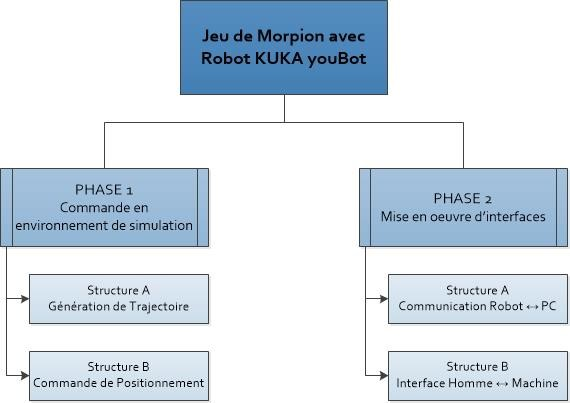
\includegraphics[width=8cm]{./diagram.jpg}
		\caption{Diagramme en arbre de la structure de découpage du projet }
		\label{fig:diagram}
	\end{center}
\end{figure}


Ci-dessous, on a défini les tâches à entreprendre en chaque structure de découpage du projet. Dans la section \ref{Methodologie} on a décrit les tâches de façon plus détaillée.
\newpage
